%%%%%%%%%%%%%%%%%%%%%%%%%%%%%%%%%%%%%%%%%%%%%%%%%%%%%%%%%%%%%%%%
%%%%%%%%%%%%%%%%%%%%%%%%%%%%%%%%%%%%%%%%%%%%%%%%%%%%%%%%%%%%%%%%
%%%%
%%%% This text file is part of the source of 
%%%% `Introduction to High-Performance Scientific Computing'
%%%% by Victor Eijkhout, copyright 2012-7
%%%%
%%%% This book is distributed under a Creative Commons Attribution 3.0
%%%% Unported (CC BY 3.0) license and made possible by funding from
%%%% The Saylor Foundation \url{http://www.saylor.org}.
%%%%
%%%%
%%%%%%%%%%%%%%%%%%%%%%%%%%%%%%%%%%%%%%%%%%%%%%%%%%%%%%%%%%%%%%%%
%%%%%%%%%%%%%%%%%%%%%%%%%%%%%%%%%%%%%%%%%%%%%%%%%%%%%%%%%%%%%%%%
\documentclass[11pt,letterpaper,twoside,openany]{boek3}
%\documentclass{book}

\usepackage{comment,verbatim}
\makeatletter
\def\verbatim@startline{\verbatim@line{\leavevmode\kern\unitindent\relax}}
\makeatother

\newif\ifIncludeAnswers
\IncludeAnswersfalse
\excludecomment{booth}
\input inex
\includecomment{gpu} % VLE time to remove this environment

\begin{notlulu}
  \usepackage[pdftex,colorlinks]{hyperref}
  \usepackage[all]{hypcap}
\end{notlulu}
\begin{lulu}
  \usepackage{url}
\end{lulu}

\usepackage{amssymb}
\usepackage[fleqn]{amsmath}
\usepackage{graphicx,undertilde,arydshln,wrapfig}
\usepackage{times,makeidx,multirow,multicol}
\usepackage{dirtree}

\usepackage[algo2e,noline,noend]{algorithm2e}
\newenvironment{displayalgorithm}
 {\par
  \begin{algorithm2e}[H]\leftskip=\unitindent \parskip=0pt\relax
  \DontPrintSemicolon
  \SetKwInOut{Input}{Input}\SetKwInOut{Output}{Output}
 }
 {\end{algorithm2e}\par}
\newenvironment{displayprocedure}[2]
 {\everymath{\strut}
  \begin{procedure}[H]\leftskip=\unitindent\caption{#1(#2)}}
 {\end{procedure}}

\def\verbatimsnippet#1{\verbatiminput{snippets/#1}}

% for edmond
\usepackage{subfigure,algorithmic,algorithm}

\def\lulurevision{2016}

%% \usepackage{minitoc}
%% \dominitoc[n]


%
% page layout
%
\usepackage{geometry}
\addtolength{\textwidth}{.5in}
\addtolength{\textheight}{.5in}
\addtolength{\evensidemargin}{-.5in}

\usepackage{fancyhdr}
\pagestyle{fancy}\fancyhead{}\fancyfoot{}
% remove uppercase from fancy defs
\makeatletter
\def\chaptermark#1{\markboth {{\ifnum \c@secnumdepth>\m@ne
 \thechapter. \ \fi #1}}{}}
\def\sectionmark#1{\markright{{\ifnum \c@secnumdepth >\z@
 \thesection. \ \fi #1}}}
\makeatother
% now the fancy specs
%\fancyhead[LE]{\thepage \hskip.5\unitindent/\hskip.5\unitindent \leftmark}
%\fancyhead[RO]{\rightmark \hskip.5\unitindent/\hskip.5\unitindent \thepage}
\fancyhead[LE]{\leftmark}
\fancyfoot[LE]{\thepage}
\fancyhead[RO]{\rightmark}
\fancyfoot[RO]{\thepage}
\fancyfoot[RE]{\footnotesize\sl Introduction to High Performance
  Scientific Computing}
\fancyfoot[LO]{\footnotesize\sl Victor Eijkhout}

\begin{booth}
  \usepackage{draftwatermark}
  \SetWatermarkText{TACC Booth Copy}
  \SetWatermarkScale{0.75}
\end{booth}

\input exmacs

\newwrite\nx
\newcommand\CHAPTER[2]{
\Level 0 {#1}\label{ch:#2}
\def\chapshortname{#2}
{\SetBaseLevel 1 \input chapters/#2
 \write\chapterlist{\chapshortname}
 \openout\nx=exercises/\chapshortname-nx.tex
 \write\nx{\arabic{excounter}}
 \closeout\nx
 \SetBaseLevel 0
}}

\newwrite\nx
\newcommand\APPLICATION[2]{
\Level 0 {#1}\label{app:#2}
\def\chapshortname{#2}
{\SetBaseLevel 1 \input applications/#2
 \write\chapterlist{\chapshortname}
 \openout\nx=exercises/\chapshortname-nx.tex
 \write\nx{\arabic{excounter}}
 \closeout\nx
 \SetBaseLevel 0
}}

\includecomment{tutorials}
\newcommand\TUTORIAL[2]{
\vfill\pagebreak \Level 0 {#1}\label{tut:#2}
\def\chapshortname{#2}\setcounter{excounter}0\relax
{\SetBaseLevel 1 \input tutorials/#2
\write\chapterlist{\chapshortname}
\openout\nx=exercises/\chapshortname-nx.tex
\write\nx{\arabic{excounter}}
\closeout\nx
\SetBaseLevel 0
}}
\newif\ifprojects\projectsfalse
\newcommand\PROJECT[2]{
\ifprojects \vfill\pagebreak \else \projectstrue \fi
\Level 1 {#1}\label{prj:#2}
\def\chapshortname{#2}
{\SetBaseLevel 2 \input projects/#2
\write\chapterlist{\chapshortname}
\openout\nx=exercises/\chapshortname-nx.tex
\write\nx{\arabic{excounter}}
\closeout\nx
\SetBaseLevel 0
}}
\newcommand\APPENDIX[3]{
  \vfill\pagebreak \Level 0 {#1}\label{app:#3}
  \def\chapshortname{#3}
  {\SetBaseLevel 1 {\index{#2|(}}
   \setcounter{excounter}0
   \input appendices/#3 {\index{#2|)}}
   \write\chapterlist{\chapshortname}
   \openout\nx=exercises/\chapshortname-nx.tex
   \write\nx{\arabic{excounter}}
   \closeout\nx
   \SetBaseLevel 0
  }
}
\newcommand\APPENDIXac[3]{
  \vfill\pagebreak \Level 0 {#1}\label{app:#3}
  \def\chapshortname{#3}
  {\SetBaseLevel 1 {\indexacstart{#2}}
   \setcounter{excounter}0
   \input appendices/#3 {\indexacend{#2}}
   \write\chapterlist{\chapshortname}
   \openout\nx=exercises/\chapshortname-nx.tex
   \write\nx{\arabic{excounter}}
   \closeout\nx
   \SetBaseLevel 0
}}

\newcommand\maillink[3]{
  \href{mailto:eijkhout@tacc.utexas.edu?subject=comment on section #1 "#2"}
    {comments on this #3?}\par
}
\renewcommand\maillink[3]{}

\usepackage{outliner}
\OutlineLevelStart0{\chapter{#1}
  \maillink{arabic{chapter} "#1"}{#1}{chapter}
}
\OutlineLevelStart1{\section{#1}
\maillink{\arabic{chapter}.\arabic{section}}{#1}{section}
}
\OutlineLevelCont1{\section{#1}
\maillink{\arabic{chapter}.\arabic{section}}{#1}{section}
}
\OutlineLevelStart2{\subsection{#1}
  \maillink
    {\arabic{chapter}.\arabic{section}.\arabic{subsection}}{#1}{subsection}
}
\OutlineLevelStart3{\subsubsection{#1}}
\setcounter{secnumdepth}{4}
\OutlineLevelStart4{\paragraph{\bf #1}}

\newcommand\heading[1]{\paragraph*{\textbf{#1}}}

\input scimacs
\input tutmacs

\makeindex
%\tracingmacros=2
%\tracingcommands=2

\def\publicdraft{{\bf\normalsize \\Evolving Copy - open for comments}}
\def\revdate{2nd edition, revision 2016}
\begin{lulu}
\def\publicdraft{}
\end{lulu}
\author{Victor Eijkhout\\ with\\Edmond Chow, Robert van de Geijn}
\title{Introduction to High Performance Scientific Computing
\publicdraft
}
\expandafter\date\expandafter{\revdate}

\newwrite\chapterlist \openout\chapterlist=chapternames.tex

\begin{document}
%\dosecttoc
\maketitle

\input copyright
\input introduction

\vfill\pagebreak 
{\setcounter{tocdepth}{1}
\tableofcontents
\setcounter{tocdepth}{2}
}

\part{Theory}

\CHAPTER{Single-processor Computing}{sequential}
\CHAPTER{Parallel Computing}{parallel}
\CHAPTER{Computer Arithmetic}{arithmetic}
\begin{comment}
\CHAPTER{Approximation}{approximation}
\end{comment}
\CHAPTER{Numerical treatment of differential equations}{odepde}
\CHAPTER{Numerical linear algebra}{linear}
\CHAPTER{High performance linear algebra}{parallellinear}

\part{Applications}

\APPLICATION{Molecular dynamics}{md}
\begin{lulu}
  \APPLICATION{Sorting}{sorting}
\end{lulu}
\begin{notlulu}
  \APPLICATION{Combinatorial algorithms}{combinatorics}
\end{notlulu}
\APPLICATION{Graph analytics}{graphalgorithms}
\APPLICATION{N-body problems}{discrete}
\begin{montecarlo}
\APPLICATION{Monte Carlo Methods}{montecarlo}
\end{montecarlo}
\begin{notready}
\APPLICATION{Computational biology}{bio}
\APPLICATION{Big data}{analytics}
\APPLICATION{Computer graphics}{graphics}
\end{notready}

% not for public consumption
\begin{notready}
\APPLICATION{Other physics applications}{lbm}
\end{notready}

\begin{comment}
%%\CHAPTER{Performance measurement and optimization}{performance}
%%\CHAPTER{Applications}{applications}
%%\CHAPTER{Scientific Programming}{programming}
\end{comment}

\part{Appendices}
\setcounter{tocdepth}{1}
%\vfill\pagebreak
%\appendix
%\makeatletter
%\renewcommand\theexcounter{\@arabic\c@section.\@arabic\c@excounter}
%\renewcommand\exercisenumber{\Alph{chapter}.\arabic{section}.\arabic{excounter}}
%\makeatother
%\addcontentsline{toc}{toc}{Appendices}

%\Level 0 {Theoretical background}

\input appendices/blurb

\APPENDIX{Linear algebra}{linear algebra}{norms}
\APPENDIX{Complexity}{complexity}{complexity}
\APPENDIX{Partial Differential Equations}{partial differential equations}{pde}
\APPENDIX{Taylor series}{Taylor series}{taylor}
\APPENDIX{Graph theory}{graph!theory}{graph}
\begin{notready}
\APPENDIX{Fourier Transforms}{Fourier Transform}{fft}
\end{notready}
\APPENDIXac{Automata theory}{FSA}{fsa}
\APPENDIX{Parallel Prefix}{prefix operation}{prefix}

\begin{tutorials}
\part{Tutorials}
%\Level 0 {Practical tutorials}
\label{app:practical}

\input tutorials/blurb
%\minitoc

\TUTORIAL{Unix intro}{unix}
\begin{notready}
  \TUTORIAL{Text editing}{editors}
\end{notready}
\TUTORIAL{Compilers and libraries}{compile}
\TUTORIAL{Managing projects with Make}{gnumake}
\TUTORIAL{Source code control}{svn}
\TUTORIAL{Scientific Data Storage}{hdf5}
\TUTORIAL{Scientific Libraries}{petsc}
\TUTORIAL{Plotting with GNUplot}{gnuplot}
\TUTORIAL{Good coding practices}{coding}
\TUTORIAL{Debugging}{debug}
\begin{notready}
  \TUTORIAL{C for high performance}{cperf}
  \TUTORIAL{Performance measurement}{performance}
\end{notready}
\TUTORIAL{C/Fortran interoperability}{language}
\TUTORIAL{LaTeX for scientific documentation}{latex}

\end{tutorials}

\part{Projects, codes, index}

\Level 0 {Class projects}

\PROJECT{Cache simulation and analysis}{cache}
\PROJECT{Evaluation of Bulk Synchronous Programming}{bsp}
\PROJECT{Heat equation}{heat}
\PROJECT{The memory wall}{wall}

\Level 0 {Codes}
\label{app:codes}
\input appendices/codes

\vfill\pagebreak

\Level 0 {Bibliography, index, and list of acronyms}

\Level 1 {Bibliography}

\bibliography{vle}
\bibliographystyle{plain}
\vfill\pagebreak

%\def\acitem#1#2{\item[#1] #2}
\def\acitem#1#2{\item[#1]{#2}\index{#1|see{#2}}}
\def\acitemi#1#2#3{\item[#1]{#2}\index{#1|see{#3}}}

%\hbox{}\vskip-1in\hbox{}

\Level 1 {List of acronyms}

\begin{multicols}{2}
\begin{description}
\input acronyms
\end{description}
\end{multicols}
\vfill\pagebreak

\Level 1 {Index}

\index{cluster!node|see{node}}
\index{CPU-bound|see{compute-bound}}
\index{directives|see{compiler, directives}}
\index{GNU!gdb|see{gdb}}
\index{halo|see{ghost region}}
\index{irreducible|see{reducible}}
\index{modified Gramm-Schmidt|see{Gram-Schmidt, modified}}
\index{parallel prefix|see{prefix operation}}
\index{Roadrunner|see{IBM!Roadrunner}}
\begin{multicols}{2}
\printindex
\end{multicols}

\hbox{}\vfill
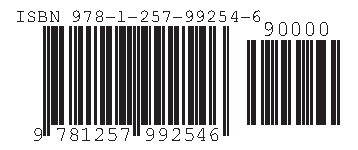
\includegraphics{isbn_barcode}

\closeout\chapterlist
\end{document}
